\begin{figure*}


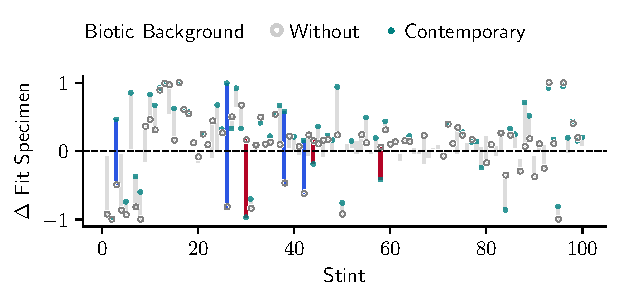
\includegraphics[width=0.51\linewidth,trim={0 1.1cm 0 0},clip]{%
binder-2025-08-24-keyfig/binder/teeplots/2025-08-24-keyfig/baseline=without+bbg=contemporary+subject=specimen+viz=signchangedotplot+ext=.pdf}%
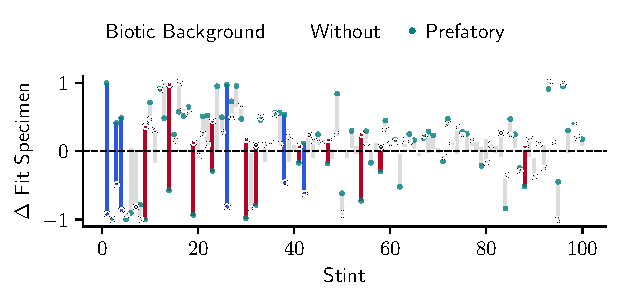
\includegraphics[width=0.45\linewidth,trim={1.2cm 1.1cm 0 0},clip]{%
binder-2025-08-24-keyfig/binder/teeplots/2025-08-24-keyfig/baseline=without+bbg=prefatory+subject=specimen+viz=signchangedotplot+ext=.pdf}

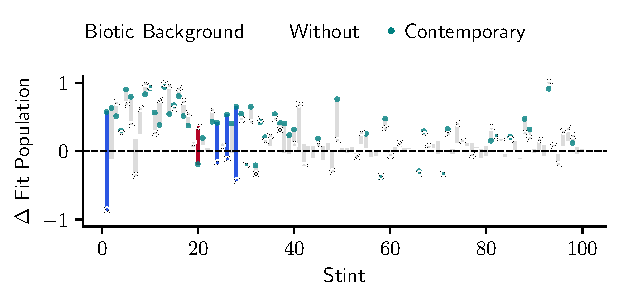
\includegraphics[width=0.51\linewidth,trim={0 0 0 1cm},clip]{%
binder-2025-08-24-keyfig/binder/teeplots/2025-08-24-keyfig/baseline=without+bbg=contemporary+subject=population+viz=signchangedotplot+ext=.pdf}%
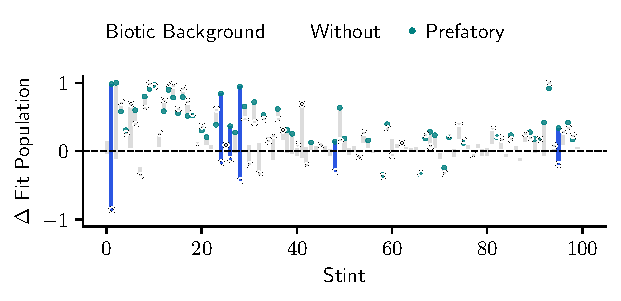
\includegraphics[width=0.45\linewidth,trim={1.2cm 0 0 1cm},clip]{%
binder-2025-08-24-keyfig/binder/teeplots/2025-08-24-keyfig/baseline=without+bbg=prefatory+subject=population+viz=signchangedotplot+ext=.pdf}

\vspace{-1ex}

\caption{
\textbf{Fitness trade-offs driven by ecological context.}
\footnotesize
Plots report influence on focal strain competition assays attributable to presence versus absence of background strain.
Experiments competed focal strain samples (specimen or population from stint $n+1$ against baseline focal strain population from stint $n$.
Outcomes recorded between $1$ (fitness gain; stint $n$ baseline driven extinct) and $-1$ (fitness loss; stint $n+1$ driven extinct), with near-zero values indicating comparable fitness.
Vertical line segments mark discrepancy between abiotic conditions (``without,'' hollow markers) and biotic conditions (filled markers).
Markers omitted where no significant significant fitness change detected between stint $n+1$ and stint $n$ baseline ($\alpha = 0.005$).
Segment color highlights sign-change effect: harmful trait becomes beneficial under ecological context (blue) or vice versa (red).
Subplots differ in focal strain sample type (rows) and source of ecological context (columns).
Under prefatory context, background strain from stint $n$; under contemporary context, stint $n+1$.
To account for possible confounding effects from resource-balancing diversity maintenance mechanism used with background strain, specimen assays were replicated with this mechanism disabled (Supplementary Figure \ref{fig:sign-change-nodmaint-vs-nodmaint}); results were generally similar (Supplementary Figure \ref{fig:sign-change-nodmaint}).
}
\label{fig:sign-change}

\end{figure*}
